\documentclass[tikz,border=4pt]{standalone}
\usepackage{xcolor}
\usetikzlibrary{arrows.meta,calc,positioning}

\definecolor{coolant}{HTML}{1F77B4}
\definecolor{heat}{HTML}{D95F02}
\definecolor{plate}{HTML}{D8DEE9}
\definecolor{solid}{HTML}{7B8794}

\begin{document}
\pagecolor{white}
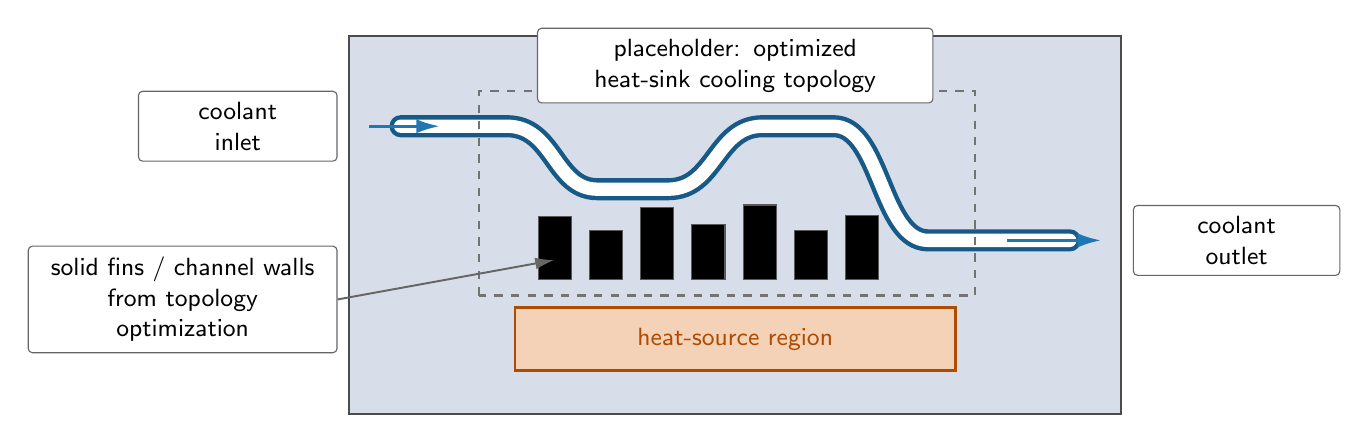
\begin{tikzpicture}[
    font=\sffamily,
    flow/.style={coolant, -{Latex[length=3.0mm,width=1.8mm]}, line width=1.1pt},
    channel/.style={coolant!75!black, line width=8pt, line cap=round, line join=round},
    note/.style={draw=black!60, fill=white, rounded corners=1.5pt,
                 align=center, inner xsep=6pt, inner ysep=4pt,
                 font=\sffamily\small},
    zone/.style={draw=black!55, dashed, line width=0.8pt}
]

\fill[plate] (0,0) rectangle (9.8,4.8);
\draw[black!70, line width=0.8pt] (0,0) rectangle (9.8,4.8);

\fill[heat!28] (2.1,0.55) rectangle (7.7,1.35);
\draw[heat!80!black, line width=0.9pt] (2.1,0.55) rectangle (7.7,1.35);
\node[font=\sffamily\small, text=heat!80!black] at (4.9,0.95) {heat-source region};

\draw[channel]
    (0.65,3.65) -- (2.00,3.65)
    .. controls (2.60,3.65) and (2.60,2.85) .. (3.15,2.85)
    -- (4.05,2.85)
    .. controls (4.65,2.85) and (4.65,3.65) .. (5.25,3.65)
    -- (6.15,3.65)
    .. controls (6.75,3.65) and (6.75,2.20) .. (7.35,2.20)
    -- (9.15,2.20);

\draw[white, line width=4.8pt, line cap=round, line join=round]
    (0.65,3.65) -- (2.00,3.65)
    .. controls (2.60,3.65) and (2.60,2.85) .. (3.15,2.85)
    -- (4.05,2.85)
    .. controls (4.65,2.85) and (4.65,3.65) .. (5.25,3.65)
    -- (6.15,3.65)
    .. controls (6.75,3.65) and (6.75,2.20) .. (7.35,2.20)
    -- (9.15,2.20);

\draw[flow] (0.25,3.65) -- (1.15,3.65);
\draw[flow] (8.35,2.20) -- (9.55,2.20);
\node[note, anchor=east, text width=21mm] at (-0.15,3.65) {coolant\\inlet};
\node[note, anchor=west, text width=22mm] at (9.95,2.20) {coolant\\outlet};

\foreach \x/\y/\w/\h in {
    2.40/1.70/0.42/0.80,
    3.05/1.70/0.42/0.62,
    3.70/1.70/0.42/0.92,
    4.35/1.70/0.42/0.70,
    5.00/1.70/0.42/0.95,
    5.65/1.70/0.42/0.63,
    6.30/1.70/0.42/0.82
}{
    \fill[solid] (\x,\y) rectangle ++(\w,\h);
    \draw[black!65, line width=0.4pt] (\x,\y) rectangle ++(\w,\h);
}

\draw[zone] (1.65,1.50) rectangle (7.95,4.10);
\node[note, text width=46mm] at (4.9,4.42)
    {placeholder: optimized heat-sink cooling topology};
\node[note, anchor=east, text width=35mm] (solidLabel) at (-0.15,1.45)
    {solid fins / channel walls\\from topology optimization};
\draw[-{Latex[length=2.4mm,width=1.5mm]}, black!60, line width=0.7pt]
    (solidLabel.east) -- (2.60,1.95);

\end{tikzpicture}
\end{document}
